\chapter{Likovno upodabljanje s potezami}
%
Likovno upodabljanje s potezami (\emph{kratica} LUP; \emph{angl.~stroke--based rendering}) je skupni pojem za likovna upodabljanja slik, pri katerih na risalno podlago na predpisan način postavljamo diskretne elemente. Diskretni elementi so lahko poteze čopiča, pike, kvadratki, mozaične ploščice \ldots

Cilj SBR je taka postavitev diskretnih elementov na risalno podlagi, ki bo zadostila našim pogojem in ciljem. Skupni cilj je, da s postavitvijo diskretnih elementov na risalno podlago skušamo ustavariti sliko, ki bo po stilu čimbolj podobna nekemu stilu oz.\ bo nosila določen slikarski stil. Po drugi strani želimo, da naša slika ne deluje preveč umetno, potrebno je tudi omejeiti na nek način število diskretnih elementov, njihovo obliko, barvo, \ldots

Algoritem v splošnem poteka v več fazah:
%
\begin{enumerate}
\item postavitev diskretnih elemntov na risalno podlago;
\item rendiranje diskretnih elementov.
\end{enumerate}
%
Najprej definirajmo pojma strokesa in podatkovno strukturo slika.
%
\begin{definicija}
Strokes je podatkovna struktura, ki jo lahko rendiramo. Model strokesa je opis strokesa, ki nosi podatke o obliki, poziciji in parametrih za njegovo rendiranje.
\end{definicija}
% 
Strokesi, ki jih bomo uporabljali mi, bodo več vrst:
%
\begin{itemize}
\item pike (model pike: radij, center, barva);
\item poteze s čopičem (enostavnejši in bolj bogat model - opisa sledita kasneje);
\item ploščice, ki potrenujemo pri mozaikih;
\item trganke (trganke iz revije).
\end{itemize}
%
\begin{definicija}
Struktura slike je podatkovna struktura, ki vsebuje:
\begin{itemize}
\item Platno, na katerega bomo slikali (barva platna in njegova struktura);
\item Urejen seznam strokesov, ki jih določajo parametri.
\end{itemize}
\end{definicija}
%
Sedaj potrebujemo še oceno, ki nam bo povedala kako dobra je struktura slike, glede na cilje, ki smo si jh zadali.
%
\begin{definicija}
SBR energijska funkcija je funkcija $\fun{E}{I}{R}$, pri čemer je $I$ množica vseh možnih struktur slike in $R$ množica relanih vrednosti.
\end{definicija}
%
Intuitivno lahko gledamo na energijsko funkcijo kot na merilo, ki nam pove, kako dobro narisana je slika. Cilj SBR-ja je naslikati sliko, ki bo imela čimmanjšo možno vrednost energije. Naš cilj pri risanju je, da bi dano sliko čimbolje narisali, torej da bo naša končna slika čimboljši približek originalne slike. To je enostavno doseči tako, da na risalno podlago naslikamo čimveč majhnih strokesov. Na ta način bomo dobili zelo dobro ujemenje. Na ta način bomo torej dobili zelo dober približek originalne slike. Ne bomo pa dosegli umetniškega cilja. Namreč, da bi poustavrili določen slikarski stil. Zato poleg zahteve, da dobimo čimboljšo ujemanje slike, dodamo zraven motnje, omejimo število strokesov, njihovo velikost itd.\ 

Z energijsko funkcijo bomo torej določili slikarski stil. Slikarski stil lahko definiramo kot sledi:
%
\begin{definicija}
SBR stil je model strokesa skupaj z energijsko funkcijo (vključujoč vrednosti parametrov) preko strukture slike.
\end{definicija}
%
Z drugimi besedami, SBR algoritem ustvari sliko z določenim stilom tako, da minimizira določeno energijsko funkcijo.

Glede na postavljanje strokesov na risalno podlago, ločimo dve glavni vrsti SBR algoritmov:
%
\begin{enumerate}
\item optimizacijski algoritmi;
\item požrešni algoritmi.
\end{enumerate}
%
V nadaljevanju si bomo pogledali algoritme iz obeh sklopov. Delo je povzeto po doktorski disertaciji od strica Hertzmanna.
%%
\section{Optimizacijski algoritmi}
%
Pri požrešni metodi smo poteze postavljali na platno po vnaprej določenem pravilu. Ko smo potezo enkrat postavili na platno, je nismo več spreminjali. Opazimo pa, da bi bilo večkrat za dosego lepše slike bolje, da bi neki potezi spremenili obliko in barvo ali pa jo celo odstranili. Tak način razmišljanja uporablja optimizacijski pristop k likovnemu upodabljanju s potezami, ki ga bomo spoznali v tem razdelku.

Najprej moramo uvesti matematično merilo, ki bo za dano trenutno postavitev potez na platnu $J$ izmerilo njeno kvaliteto.
%
\begin{definicija}
\emph{LUP energijska funkcija} je funkcija $\fun{E}{\J}{\R}$, kjer je $\J$ množica vseh možnih slik.
\end{definicija}
%
Glavni dve merili, ki ju bomo upoštevali pri računanju vrednosti energijske funkcije, sta število potez in ujemanje slike $J$ z vhodno sliko $I$. Seveda bi lahko z ogromnim številom majhnih potez zelo dobro aproksimirali vhodno sliko $I$, vendar pa ne bi dobili likovno zadovoljivega rezultata. Pri optimiziranju skušamo doseči, da neko sliko aproksimiramo z manjšim številom potez. Na ta način v sliko vnesemo abstrakcijo in željeni likovni pridih. Osnovna energijska funkcija, ki jo bomo optimizirali, bo:
%
\begin{align*}
E(J) & = E_p(J) + w_n \cdot E_n(J), \\
E_p(J) & = \sum_{(x, y) \in J} \norm{J(x, y) - I(x, y)}^2, \\
E_n(J) & = \textup{število potez na sliki }J.
\end{align*}
%
S parametrom $w_n$ nadziramo abstrakcijo slike. Uporaba majhne vrednosti parametra $w_n$ pomeni, da bomo pri slikanju uporabili veliko število potez, posledično bomo dobili likovna dela, ki bodo verjetno bolj ali manj podobna začetni vhodni sliki $I$. Za dosego bolj likovno estetskega rezultata bomo torej običajno uporabljali večje vrednosti parametra $w_n$, saj bomo na ta način zmanjšali število končnih potez.

Izbira energijske funkcije, ki jo bomo uporabili pri optimiziranju, skupaj z modelom poteze določa \emph{stil slike}. Določen stil slike dobimo torej tako, da minimiziramo energijsko funkcijo.
%
\begin{opomba}
Energijsko funkcijo lahko izberemo tudi kot merilo za kvaliteto sliko, ki jo dobimo pri slikanju s požrešno metodo.
\end{opomba}
%
Kljub temu, da bomo pri slikanju na optimizacijski način dobili veliko boljši rezultat kot pri požrešni metodi, pa tak način slikanja ni naraven. Slikar namreč na platnu ponavadi neke poteze, ko jo naslika na platno, običajno ne more več spreminati. Minus je tudi ta, da bo čas likovnega upodabljanja v nekaterih primerih drastično narastel (če bi pri požrešni metodi porabili pet minut, se kaj lahko zgodi, da bomo pri optimiziranju za dosego podobnega stila pri isti vhodni sliki potrebovalii pet ur). Optimizacijski pristop po drugi strani pri svojem ustvarjanju uporabljajo sestavljalci mozaiki. Sestavljalec najprej na podlagi s prestavljanjem, izbiro ploščiš druge barve in spreminjanjem oblike ploščic sestavi željeno sliko, nato pa ploščice zacementira.

V podrazdelkih, ki sledita, bomo opisali dva optimizacijska pristopa. Prva skupina algoritmov, ki jo bomo opisali, so Voronojevi algoritmi. Z njimi bomo pokazali kako lahko sestavimo mozaik. Nato bomo spoznali še izkustvene algoritme, pri katerih bomo uporabljali hevristično izbrane teste, s pomočjo katerih bomo minimizirali energijsko funkcijo. Voronojevi algoritmi imajo boljšo časovno zahtevnost, ampak je ne moremo prilagoditi različnim vrstam problemov. Medtem ko imajo izkustveni algoritmi slabšo časovno zahtevnost, pa jih lahko z izbiro energijske funkcije in parametrov prilagodimo različnim problemov in poustavrimo veliko več likovnih stilov.
%
%% Voronojevi diagrami
\subsection{Voronojevi algoritmi}
%
Pri razvoju Voronjevega algoritma za LUP, si bomo pomagali z znanjem računske geometrije. V primeru, ko bomo na podlago postavljali neprekrivajoče se poteze s podobno obliko, bomo videli, da lahko problem prevedemo na znan Voronojev diagram. Metoda, ki jo bomo predstavili v našem delu, je bila preedstavljena v članku \cite{Hausner}.
%
\subsubsection{Lloydova metoda}
Množico enakomerno razporejenih diskretnih elementov na risalni podlagi bomo določili s pomočjo iterativnega optimizacijskega postopka, ki bo minimiziral predpisano energijsko funkcijo. Naj bo $p = (x, y)$ slikovna točka in označimo s $C_i$ posebno slikovno točko, ki ji pravimo \emph{center}. Diskretne elemente bomo postavili na sliko tako, da bodo imeli središča v centrih. Naj bo $L_p^i \in \set{0, 1}$ označitev slikovnih točk, pri čemer $L_p^i = 1$ pomeni, da slikovna točka $p$ pripada centru $C_i$. Vsaka slikovna točka pripada natanko enemu centru, veljati mora $\sum_p L_p^i = 1$.

\textbf{Naloga:} Izbira množice centrov in označitve slikovnih pik, ki minimizira naslednjo energijsko funkcijo \footnote{Pri NPR-ju velikokrat namesto diskretne verzije izberejo zvezno verzijo problema. Ker pa je diskretni problem bližje realnemu problemu in za ta primer lahko pokažemo konvergenco algoritma, bomo mi izbrali diskretno verzijo problema.}:
%
\begin{align*}
E(I) & = \sum_{p \in I} L_p^i \norm{p - C_i}^2 \\
       & = \sum_{p \in I} L_p^i ((p_x - C_{i, x})^2 + (p_y - C_{i, y})^2) .
\end{align*}
%
Z drugimi besedami, vsaki slikovni točki želimo pripisati center, ki ji je najbližji. Če bi poznali množico centrov vnaprej, bi optimalno označitev enostavno izračunali tako, da bi vsaki slikovni točki pripisali njej najbližji center. Slednjo nalogo poznamo pod imenom Voronojev diagram. Več o Voronojevem diagramu si lahko preberemu v \cite{voronoi}.

Kot je razvidno iz slike \ref{slika1a}, naključna izbira centrov ne bo dala zadovoljivega rezultata. Izboljšava, ki jo lahko naredimo je ta, da spremenimo položaje centrov. Energijsko funkcijo želimo optimizirati samo glede na množico centrov, zato moramo rešiti enačbo $\frac{\partial E(I)}{\partial C_i} = 0$. Nove položaje centrov izračunamo torej po formuli
%
$$C_i = \frac{\sum_p L_p^i p}{\sum_p L_p^i}.$$
%
Zgornja formula nam da srednjo vrednost vseh položajev slikovnih točk, ki smo jih na začetku pripisali določenemu centru. Zatem, ko spremenimo množico centrov, zopet na novo izračunamo označitev. Ponavljanje zgoraj opisanih korakov poznamo pod imenom Lloydova metoda. Psevdokoda Lloydeve metode je predstavljena v algoritmu \ref{alg:Lloyd}.
%
% TODO Algoritem
%
Na sliki \ref{slika1b} je prikazana množica centrov in Voronojev diagram po tem, ko na prvotni množici centrov uporabimo Lloydovo metodo. Pravimo, da zgornji algoritem konvergira, ko se vrednost energijske funkcije med posameznima korakoma optimizacije ničveč ne spreminja. na vsakem koraku se bo vrednost energijske funkcije kvečjemu zmanjšala, saj na vsakem koraku energijsko funkcijo minimiziramo glede na določene parametre. Metoda bo zagotova konvergirala, saj je na voljo le končno mnogo kombinacij množic centrov in označitev slikovnih pik, na vsakem koraku pa se vrednost energijske funkcije kvečjemu zmanjša.
% TODO Tukaj še povej, da je to počasi pa nekaj kdo je to odkril, pa da je hardware pomemben za hitrost.
\subsubsection{Prilagojena Lloydova metoda za reševanje problema SBR}
Sedaj, ko imamo na voljo algoritem, ki nam enakomerno razporedi centre na sliki, lahko Lloydovo metodo prilagodimo tako, da jo bomo uporabili za rešitev problema SBR. Najosnovnejši problem SBR, ki ga obravnavamo je taka postavitev točk na sliko, ki bo čimbolje aproksimirala dano črnobelo sliko. Za ta problem obstajajo že rešitev % TODO
Poglejmo si rešitev, ki jo je predstavil \ref{Sec02}. Namesto, da spreminjamo velikost narisanih točk, spreminjamo njihovo gostost. Uporabili bomo funkcijo ploskovne gostote $\rho(p)$, ki bo določala gostost točk na posameznih območjih vhodne slike. Funkcijo ploskovne gostote izpeljemo iz vhodne slike $T(p)$, ki smo jo predhodno pretvorili v črnobelo, po formuli
$$\rho(p) = 1 - \frac{T(p)}{m},$$
kjer je $m$ največja vrednost slike $T$. Nova energijska funkcija za ta problem se glasi
%
\begin{align*}
E(I) & = \sum_{p \in I} L_p^i \rho(p) \norm{p - C_i}^2 \\
       & = \sum_{p \in I} L_p^i \rho(p) ((p_x - C_{i, x})^2 + (p_y - C_{i, y})^2).
\end{align*}
%
Podoben razmislek kot pri navadni Lloydovi metodi nas pripelje sedaj do nekoliko spremenjene Lloydove metode. Postopek označitve slikovnih točk ostane isti kot prej. Ker smo vsaki točki s funkcijo ploskovne gostote pripisali utež, moramo pri računanju novih centrov te uteži upoštevati. Namesto običajne srednje vrednosti, bomo torej morali za posamezne centre vzeti uteženo povprečje slikovnih točk iz pripadojoče celice. Nove centre izračunamo po formuli
%
$$C_i = \frac{\sum_p L_p^i \rho(p)p}{\sum_p L_p^i \rho(p)}.$$
%
Računanje novih centrov lahko pohitrimo tako, da vsote uteži, ki nastopajo v imenovalcih, izračunamo vnaprej. S to metodo dobimo ostrejše robove na sliki, saj je gostota točk odvisna od tonske slike. % TODO Secord je uporabljal tudi neko drugo določitev začetnih točk.

Lloydovo metodo pa lahko uporabimo tudi za sestavljanje mozaikov na podlagi dane barvne vhodne slike. Preprosti pristop, ki ga lahko uporabimo pri mozaiku je, da izračunamo Voronojev diagram in za barve posameznih celic uporabimo barvo, ki jo ima center na vhodni sliki. Ta pristop ni najbolšji, saj pri njem dobimo mozaik, ki ima preveč nepravilne oblike ploščic.

Hausner \ref{Hau01} opisuje dve izpopolnitvi metode. Najprej naodmestimo evklidsko razdaljo oz.\ $L_2$ normo z $L_1$ normo ($\norm{v}_1 = \abs{v_x} + \abs{v_y}$). Druga izboljšava je določitev vektorskega polja $\Phi(p)$ sliki, da dobimo konsistentno orientacijo ploščic pri končnem mozaiku. Na ta način ploščicam v mozaiku pripišemo smer, $\phi_i = \Phi(C_i)$. Nova energijska funkcija je enaka
%
\begin{align*}
E(I) = \sum_{p \in I} L_p^i \norm{R_{\Phi(C_i)} (p - C_i)}_1^2,
\end{align*}
%
kjer je $R_{\Phi(C_i)}$ rotacijska matrika s smerjo $\Phi(C_i)$. Psevdokoda novega algoritma je povzeta v \ref{}.
% TODO Algoritem TileMosaic
%
Zgornji algoritem ni več optimizacijski, kajti posamezen korak pri optimizaciji ne bo dal nujno boljše rešitve. Še več, zgornji algoritem pri postavitvi ploščic ne upošteva barve ploščic, temveč barvo ploščicam priredi šele, ko so znani končni položaji ploščic. Čeprav teoretično izgleda, da algoritem ni najboljši, pa se v praksi izkaže, da z njim dobimo zadovoljivo dobre rezultate.

Tlakovanje lahko prilagodimo tako, da ročno razdelimo območja slike in posamezna območja tlakujemo neodvisno (izberemo lahko različne parametre, npr.\ velikosti ploščic). Iz prvotne slike lahko odstranimo tudi robove, na ta način se izognemo temu, da bi ploščica imela center na katerem izmed robov, kajti to poslabšuje kvaliteto mozaika.
%
\subsection{Izkustveni algoritmi}
Voronojev algoritem se ne da lahko razširiti tako, da bi upošteval tudi barvo ploščic in obravnaval dejstvo, da se lahko diskretni elementi tudi prekrivajo. Trenutno so edini algoritmi, ki znajo upoštevati tudi to, \emph{izkustveni algoritmi}. Izkustevni algoritem lahko uporabimo za reševanje kateregakoli SBR problema.

\textbf{Ideja:} Na vsakem algoritmu je predlagana nova sprememba za že postavljeno strukturo. V primeru, ko je sprememeba takšna, da zmanjša vrednost energijski funkciji, sprememebo izvedemo, sicer jo zavržemo.

Če je sistem, ki predlaga na vsakem koraku algoritma novo spremembo, dobro zasnovan, potem bo algoritem konvergiral k rešitvi, ki bo imela nizko vrednost energijske funkcije. Zagotovila, da bomo prišli do take rešitve, pa pri tem novem algoritmu nimamo. Prav tako nimamo zagotovila, da bomo prišli do primerne rešitve v nekem zadovoljvio majhnem času. V algoritmu \ref{trialanderror} je povzeta psevdokoda za izkustveni algoritem.
%
% TODO algoritem za izkustveni alg
%
V zgornjem algoritmu pri zanki nismo uporabili določenega zaustavitvenega pogoja, namreč pustimo, da zaustavitveni pogoj določi uporabnik. Glavna naloga pri tem algoritmu je, da postavimo dober sistem za predlaganje sprememb. Naključna izbira novih sprememb bi povzročila trošenje časa za to, da bi sistem predlagal rešitve, ki ne bi ničesar doprinesle k boljšemu rezultatu. Zato je bolje, da vzpostavimo polavtomatičen sistem, v katerem lahko uporabnik predlaga nove spremembe. Izkustevni algoritmu so v resnici podobni požrešnim algoritmom, pri obojih namreč za boljši rezultat uporabimo polavtomatiziran sistem. Kakorkoli, pri izkustvenem algoritmu se bo sprememba zgodila le, če bo nova sprememba doprinesla k boljšemu rezultatu. Pri izkustvenem algoritmu torej ni potrebno poskrbeti za to, da algoritem avtomatično ustvari nov diskretni element, ki bo pripomogel k boljšemu mozaiku.

Haeberli \ref{Hae90} je predstavil prvi izkustveni algoritem za likovno upodabljanje slik. Na vsakem koraku je izvedel spremembe določenega števila diskretnih elementov, izvedene spremembe nato ohrani, če je vsota kvadratov razlik glede na vhodno sliko zmanjšana.   
%
\subsubsection{Slikovno renderiranje z izkustvenim algoritmom}
Heartzman je izkustveni algoritem uporabil za slikovno renderiranje. Naloga je poiskati sliko, ki se bo čimbolje ujemala z vhodno sliko, bo v celoti pokrita z barvo in bo uporabljala čimmanj potez. Vsaka poteza je definirana z debelino čopiča in seznamom kontrolnih točk. Energijska funkcija, ki jo bomo minimizirali je dana z
%
\begin{align*}
E(I) & = E_{app}(I) + E_{nstr}(I) + E_{cov}(I), \\
E_{app}(I) & = \sum{p \in I} w_{app}(p) \norm{I(p) - S(p)}, \\
E_{nstr}(I) & = w_{nstr} \cdot \textup{(število potez v $I$)}, \\
E_{cov}(I) & = w_{cov} \cdot \textup{(število nepobarvanih slikovnih točk v $I$)}.
\end{align*}
%
Zgornja energijska funkcija je linearna kombinacija treh drugih energijskih funkcij, ki uravnavajo posamezne zahteve. Prva funkcija $E_{app}$ nam pove koliko nova slika aproksimira vhodno sliko $S$. Število potez v drugi funkciji $E_{nstr}$ poskrbi, da število potez na sliki ni preveliko, zahteva je namreč čimmanjše število potez. Tretja funkcija $E_{cov}$ pa poskrbi za to, da nimamo na sliki nepobarvanih slikovnih točk. Uteži $w_{app}, w_{nstr}$ in $w_{cov}$ so parametri, ki jih lahko določi uporabnik. Uteži $w_{app}$ uporabnik določi tako, da predlaga uteženo sliko, iz katere preberemo vrednosti uteži za posamezno slikovno točko.

Prvi dve funkciji uravnavata dve med sabo tekmovalni zahtevi: prva želi, da naredimo čimboljšo aproksimacijo prvotne slike, druga pa želi uporabiti čimmanj potez in s tem tudi čimamnj barve. Z uravnavanjem teh dveh parametrov lahko uporabnik doseže različne slikarske stile.

V primeru, ko uporabnik ne predlaga utežene slike, bo algoritem za uteži $w_{app}$ izbral vrednosti, ki jih bo prebral iz binarne slike, ustvarjene s pomočjo Sobelovega filtra. ta način da poseben poudarek na robove slik, kljub temu, da dobimo zadovoljive rezultate tudi, če bi uporabili kar konstantno utež skozi celotno sliko. Če dovolimo, da se vrednost parametra $w_{app}$ spreminja skozi sliko, potem dobimo efekt, ki je podoben efektu, da imamo na različnih območjih slike drugačno energijsko funkcijo. Slika uteži $w_{app}(p)$ nam dovoljuje, da nadzorujemo koliko detajlov želimo na posameznih delih slike.

% TODO Za nadaljne informacije glej doktorat oziroma nek članek paint by relaxation \ref{Her01}. 
\textbf{Relaksacija poteze:} Osnovna strategija, ki jo uporabimo za sistem predlaganja novih sprememb, je uporaba \emph{relaksacija poteze}. Gre za adaptacijo snakes \ref{10, 2} na energijsko funkcijo: poišče aproksimacijo lokalnega minimuma za dani položaj poteze.

High-level algoritem za modifikacijo poteze je:
%
\begin{enumerate}
  \item Izračunamo energijo slike.
  \item Izberemo eno izmed obstoječih potez.
  \item Po potrebi spremenimo parametre poteze.
  \item Relaksacija poteze.
  \item Izračunamo novo energijo slike.
\end{enumerate}
%
Podrobnosti implementacije so v poglavju 8.1. Na tem mestu omenimo naslednja dva aspekta implementacije:
%
\begin{itemize}
  \item Pri postopku iskanja poteze izračunamo energijo slike brez te poteze. Na ta način je lahko predlagana sprememba brisanje poteze brez dodatnega stroška.
  \item Postopek relaksacije bi bil zelo drag postopek in težek za implementacijo, če bi ga naredili eksaktno. Namesto tega uporabimo aproksimacijo za računanje energije zunaj relaksacijske zanke in izračunamo eksatno vrednost energije, ko je sprememba predlagana.
\end{itemize}
%
\textbf{Opis individualnih postopkov za generiranje spremembe:}
%
\begin{itemize}
  \item Dodajanje nove poteze: na podlagi izbrane točke na sliki ustvarimo novo potezo. Novo potezo vedno dodamo na konec seznama vseh potez (poteze narišemo na platno v vrstenm redu). Na način, ki je opisan v \ref{9} dodamo nove kontrolne točke. Novo potezo nato relaksiramo. Rezultat tega iskanja je nato predlog za novo spremembo na sliki.
  \item Reaktivacija poteze: Dana poteza je relaksirana in sprememeba je nov predlog. Vendar pa v primeru, ko bi brisanje poteze iz slike energijo slike zmanjšajo bolj kot modifikacija poteze, potem potezo pobrišemo. Brisanje ene poteze ne vpliva na vrstni red potez. Na ta način bomo v postopku pobrisali poteze, ki so zadaj za ostalimi potezami, če za vključitev poteze na sliko obstaja kazen (tj.\ $w_{area} > 0$ ali $w_{nstr} > 0$).
  \item Odebelitev poteze: Če je radij poteze pod maksimumom, potem povečamo njen radij. Potezo zatem reaktiviramo. To potezo sedaj damo kot nov predlog za spremembo.
  \item Zoožanje poteze: Če je radij poteze nad minimumom, potem radij poteze zmanjašamo in potezo reaktiviramo.
  \item Prebaravanje: Barvo poteze nastavimo na povprečno vrednost barv območja vhodne slike, ki ga obsega poteza. Potezo nato reaktiviramo.
\end{itemize}
%
\textbf{Kombinacija korakov:} Individualne spremembe kombiniramo v zanke, da zagotovimo, da je vsaka poteza vsaj enkrat relaksirana.
%
\begin{itemize}
  \item Postavitvena plast: Zanka preko slike, znotraj katere s pomočjo postopka \textit{Dodajanje poteze} dodamo novo potezo s predpisanim radijem in naključno spremenjeno začetno točko.
  \item Splošna reaktivacija: Iteracija preko množice vseh potez v njihovem zaporedju in njihova \textit{Relaksacija}.
  \item Odebeljenje/Zoožanje vseh potez: Za vsako potezo izvedemo postopek \textit{Odebelitve} dokler sprememba ni zavržena li pa poteza pobrisana. V primeru, ko poteza ostane nespremenjena izvedemo postopek \textit{Zoožitve} dokler ta sprememba ni zavrnjena lai pa poteza pobrisana.
  \item Splošno prebarvanje: Iteriramo preko množice potez in uporabimo postopek \textit{prebarvanje}.
  \item Skripta: Izvedi zaporedje relaksacijskih zank. Če želimo narediti sliko na novo, uporabimo naslednji algoritem:
% TODO algoritem
\end{itemize}
%
Običajno je $N=2$. Zgornja skripta običajno pripelje do konvergence. Opazimo, da relaksacijsko zanko izvedemo na vseh potezah, ne le teh, ki imajo trenutno velikost.
% TODO Zahtevnost.
%%
\section{Požrešne metode}
Požrešne metode so najbolj običajni algoritmi s katerimi slikamo. Strokese dodamo na strukturo slike in jih po tem ne spreminjamo več, kot smo to storili pri optimizacijskih algoritmih. Pri tej vrsti lagoritma nimamo energijske funkcije, ki bi dolačala stil slike, temveč moramo na pravi način postaviti strokese na strukturo slike. Seveda lahko zapišemo energijsko funkcijo, ki je naravna.

Dve glavni vprašanji, ki ju imamo pri požrešni metodi slikanja, sta:
%
\begin{enumerate}
\item Kam postavimo strokese?
\item Kakšno obliko in barvo bodo imeli strokesi?
\end{enumerate}
%
Pogledali si bomo različne vrste postavljanja strokesov na platno:
%
\begin{enumerate}
\item ravni strokesi (enoplastno, večplastno);
\item Bezierovi strokesi.
\end{enumerate}
%
\subsection{Slikanje z ravnimi potezami}
\subsubsection{Generiranje potez}
Privzemimo, da je vsaka poteza čopiča renderirana z antialiazirano črto s centrom v $(cx, cy)$, dano dolžino $l$, debelino čopiča $R$ in orientacijo $\theta$. Privzemimo, da so poteze čopiča generirane s centri v $(cx, cy)$ na mreži slike, ki ima v $x$ in $y$ smeri stolpce in vrstice narazen za dve slikovni točki. Na ta način zagotovimo, da bo celotno platno prekrito z barvo oz.\ potezami čopiča. V praksi uporabniku dovolimo, da nastavi razdalje. Na začetku bomo privzeli, da je orientacija konstantna, izbrali bomo $45 \circ$. Barva poteze je izbrana tako, da bilinearno interpoliramo barvno na vhodni sliki na točko $(cx, cy)$ (imamo bravno lestvico $[0, 255]$). Poteze čopiča narišemo v naključnem vrstnem redu, da se izogmnemo regularnosti in pridobimo večji občutek naravnega procesa slikanja.
%
\subsubsection{Naključne perturbacije}
Dodajanje naključnih perturbacij k parametrom poteze, pomaga pri občutku, da je poteza narisana ročno. Naključnost dolžine in debeline poteze čopiča dosežemo s tem, da uporabnik za dolžino in debelino poteze čopiča predpiše interval dovoljenih vrednosti. barvo perturbiramo tako, da komponentam RGB dodamo vrednosti $\Delta r, \Delta g$ in $\Delta b$ iz intervala $[-15, 15]$. Perturbirano barvo nato skaliramo z naključno vrednostjo $\Delta inteziteta$ iz intervala $[0.85, 1.15]$. Potem, ko dobimo končno perturbirano barvo, jo preslikamo nazaj na interval $[0, 255]$. Perturbiramo tudi orientacijo poteze, tako da orientaciji dodamo naključno vrednost iz intervala $[-15 \circ, 15 \circ]$.
%
\begin{opomba}
Dovoljene vrednosti za perturbacijo so izbrane na podlagi empiričnih poskusov.
\end{opomba}
%
\subsubsection{Rezanje in upodabljanje potez čopiča}
Potezo čopiča upodobimo tako, da narišemo antialiazirano črto skozi predpisan center v določeni orientaciji. Ker želimo ohraniti detajle in oblike na vhodni sliki, poteze čopiča porežemo pri sekanju z robovi na vhodni sliki. Na ta način se robovi na vhodni sliki bolj ali manj ohranijo. To dosežemo tako, da pričnemo v centru poteze in potezo rišemo toliko časa, dokler ta ne seka roba na vhodni sliki.

Algoritem za opis rezanja potez čopiča in njihovega upodabljanja:
%
\begin{enumerate}
  \item Iz prvotne vhodne slike izračunamo matriko, v kateri za posamezno slikovno točko hranimo njeno inteziteto. Inteziteto za slikovno točko, ki ima komponente RGB na intervalu $[0, 255]$, izračunamo njeno inteziteto s formulo:
$\frac{30\cdot r + 59 \cdot g + 11\cdot b}{100}$.
  \item Dobljeno sliko $I$ sedaj zameglimo z uporabo Gaussovega filtra. S tem filtrom na sliki zmanjšamo šum. Večji filter bo odstranil šum, vendar pa bo pri tem zameglil tudi detajle in robove na vhodni sliki. Manjši filtri pa bodo detajle in robove bolje ohranili, vendar ne bomo na ta način odstranili neželjenega šuma na sliki. Namesto Gaussovega filtra, lahko uporabimo aproksimacijo z $B$-zlepki. Uporabniku dovolimo, da nastavi ustrezne parametre.
  \item Dobljeno zamegljeno sliko sedaj filtriramo s Sobelovim filtrom. Za vsako slikovno točko izračunamo gradient $(G_x, G_y)$ in dobimo vrednost Sobelovega filtra za to slikovno točko kot
$Sobel(x, y) = Magnitude(G_x, G_y)$.
Dobimo novo sliko $S$.
  \item Za dani center $(c_x, c_y)$, orientacijo poteze $\theta$ in filtrirane slike $S$, moramo sedaj izračunati še začetno in končno točko poteze ($(x_1, y_1)$ in $(x_2, y_2)$). Postopek pričnemo v centru $(c_x, c_y)$ in rišemo potezo v določeni smeri, dokler ne dosežemo največje dovoljene dolžine ali pa sekamo rob na sliki $S$. Rob na sliki je bil najden, če vrednost graideinta oz.\ vrednost na sliki $S$ pade v smeri risanja poteze. V algoritmu \ref{alg:clipping} je prikazana psevdokoda za postopek iskanja začetne in končne točke poteze.
%
\begin{algorithm}
  \caption{Iskanje začetne in končne točke poteze. Center poteze je dan s točko $(c_x, c_y)$, smer pa je dana z $d_x, d_y$. Izhodni podatki algoritma sta začetna in končna točka ($(x_1, y_1)$ in $(x_2, y_2)$. Filtrirano sliko $S$ pregledamo v enotskih korakih dokler ne sekamo roba ali dosežemo največje dolžine poteze. Spodnji postopek je prikaz za iskanje enega konca poteze. Za vsak konec namreč moramo iti v nasprotnih smereh pri risanju. Za iskanje točke $(x_2, y_2)$ moramo tako nastaviti smer na $(d_x, d_y) = (-d_x, -d_y)$.}
  \label{alg:clipping}
\begin{algorithmic}[1]
  \State $(x_i, y_i)$ $\leftarrow$ $(c_x, c_y)$
  \State $vred$ $\leftarrow$ bilinearna vrednost filtrirane vrednosti slike $S$ v točki $(x_i, y_i)$
  \State $(x_t, y_t)$ $\leftarrow$ $(x_i + d_x, y_i + d_y)$
  \If {$d((x_i, y_i), (x_t, y_t)) > \frac{l}{2}$}
    \State $stop$
  \EndIf
  \State $vred_n$ $\leftarrow$ bilinearna vrednost filtrirane vrednosti slike $S$ v točki $(x_t, y_t)$
  \If {$vred_n < vred$}
    \State $stop$
  \EndIf
  \State $(x_i, y_i)$ $\leftarrow$ $x_t, y_t$
  \State $vred$ $\leftarrow$ $vred_n$
  \State $goto\ 3$ 
\end{algorithmic}
\end{algorithm}
%
  \item Potezo čopiča upodobimo z izračunano začetno in končno točko. Za barvo poteze izberemo kar barvo slikovne točke s koordinatami $(c_x, c_y)$ na vhodni sliki. Perturbirati moramo barvo, parametre za perturbacijo imamo shranjene. Poteze upodobimo z antialiazirano črto, i ima okrog območje linearnega padca debeline slikovne pike in spremeni prosojnost od 1 do 0. Pri upodabljanju poteze poskrbimo tudi za to, da narisana črta ni čisto točno odrezana pri koncu, temveč gre nekoliko preko robnih točk. Na ta nain dosežemo boljši učinek ročno narisane črte. Na koncih črte lahko po želji narišemo tudi krogec, da dobimo črto, ki je na koncih zaobljena ali pa pustimo ravno odrezano črto.
\end{enumerate}
%
\subsubsection{Tekstura čopiča}
Poteze čopiča lahko upodabljamo tudi s pomočjo teksture, tj.\ vzorca, ki vsebuje informacije o komponentah RGB in prosojnosti (alfa komponenta). Predpišemo padec, ki je odvisen od padca pri risanju antialiazirane črte, in ustvarimo pravokotnik, ki pokriva antialiazirano črto. Teksturo poteze čopiča preslikamo na ta pravokotnik. Posamezne barve na potezi čopča pomnožimo s temi barvami, ki so na teksturi poteze čopiča.
% TODO Skica.
\subsubsection{Usmerjenost potez čopiča}
Namesto predpisane orientacije poteze bomo izračunali orientacijo, ki bo sovpadala z linijami na slikami. Poteze tako rišemo v smeri konstantne ali skoraj konstantne barve. To orientacijo lahko aproksimiramo tako, da rišemo poteze v smeri normale na gradient slike $I$. Namreč, gradient nam pove v kateri smeri se slika najbolj spremeni, normala na gradient je torej smer v kateri se ne spremeni slika. Upoštevajoč to informacijo, pričakujemo, da lahko sliko lokalno avtomatično aproksimiramo z realtivno kratkimi potezami konstantne barve v smeri normale na gradient.

Eksperimentalno se izkaže, da uporaba istega Gaussovega filtra za detekcijo robov na sliki in zamegljenje slike za računanje gradienta ni optimalno. Izračunani gradient namreč ni bil dovolj gladek. Za izračun orientacije zato uporabimo večji Gaussov filter: uporabili so Gaussov filter, ki je bil za 4 slikovne pike večji od filtra za določanje robov.

Kakorkoli, v primeru, ko je magnituda gradienta blizu 0, se ne moremo zanesti na to, da bi bila določena smer uporabna. Zato uporabimo novo tehniko, ki spremeni gradientno polje tako, da poteze čopiča v območjih slike s konstantno ali skoraj konstsntno barvo gladko interpolirajo smeri, ki jih določajo robovi tega območja.

Najprej izločimo vrednosti gradienta na sliki, za katere velja, da je $Mag(G_x, G_y)$ blizu 0; primerna izbira je, da ven izločimo tiste gradiente, za katere velja $\abs{G_x} < 0.3$ in $\abs{G_y} < 0.3$. Izločene gradiente moramo sedaj nadomestiti z novimi vrednostmi, ki bodo dale zadovoljivo smer. To storimo tako, da interpoliramo okoliške vrednosti, ki so dobre. Ker pa dobre vrednosti ne ležijo nujno na mreži, ne moremo uporabiti kubične interpolacije na teh točkah. Zato potrebujemo interpolant, ki ne bo zahteval enakomerne razporeditve podatkov v $x$ in $y$ smereh. Uporabimo lahko interpolacijo s tankoploskovnim filtrom \ref{Franke79}.

Končno, za vsak center $(c_x, c_y)$ poračunamo vrednosti gradienta s kubično interpolacijo. Kot poda katerim narišemo potezo, izračunamo z $\arctan(\frac{G_y}{G_x}) + 90\circ$. Slednje kote nato še perturbiramo. Uporaba normale na gradient nam da efekt, da so poteze čopiča prilepljene na objekt.
% TODO Videjo.
%%
\subsection{Slikanje z Beizerovimi krivuljami}
\subsubsection{Spreminjanje velikosti čopičev}
Pogosto slikarji slikasjo tako, da najprej z debelejšim čopič naredijo grobo skico, nato pa z vedno manjšimi čopiči dodajo podrobnosti nas liko in delajo potrebne popravke. Čeprav ta postopek nima motivacije, ki bi bila vezana na računalniške algoritme, pa nam vrača estetsko primerne rezultate. Slikar tako lahko npr.\ uporablja drugčno tehniko, debelino čopiča \ldots, da naslika različne elemente na sliki (npr.\ zajčki na jasi). Uporaba potez iste oblike in barve na konstantnih območjih slike povzročijo to, da izgleda to območje umetno. V izogib temu slikar preko že narisanih potez, naslika manjše poteze, ki razgibajo sliko in poudarijo podrobnosti na sliki, ki jih slikar želi izpostaviti. Pri našemu postopku slikanja bomo z manjšim čopičem slikali le tam, kjer bo potrebno in ne povsod. Algoritem, ki ga bomo uporabljali je podoben piramidnemu algoritmu \ref{3}, pri katerem pričnemo z grobo skico in nato dodajamo detajle z vedno manjšimi čopiči. Algoritem, ki ga bomo izpeljali, v resnici temelji na Laplaceovi piramidi: diferenčna slika $L_i$ določa položaje potez čopiča. Kakorkoli, diferenčna slika predvidi popolno rekonstrukcijo na nižjih ravneh piramide, naša rekonstrukcija pa je namerno nepopolna. Zato popravki na višjih ravneh povzročijo nezaželene artefakte. Algoritem, ki ga bomo predstavili, se temu problemu izogne tako, da diferenčno sliko izračuna na novo vsakič, ko uporabimo novo debelino čopiča.

Algoritem za vhodne podatke dobi sliko in seznam debelin čopiča. Debeline čopičev določimo z njihovimi polmeri $R_i$. Algoritem nato prične s slikanjem posameznih plasti, za vsak polmer čopiča svojo. Plasti barvamo od najdebelješega čopiča proti najtanjšemu. Osnovna plast je platno, pobarvano s konstantno barvo \footnote{Platno ima lahko teksturo.}.

Za vsako plast $P_i$ najprej ustvarimo referenčno sliko, ki jo dobimo tako, da zameglimo vhodno sliko (Gaussov filter s standardnim odklonom $f_{\sigma} R_i$), kjer je $f_{\sigma}$ vnaprej določen parameter. Referenčna slika je sedaj slika, ki jo želimo čimbolje aproksimirati s čopičem trenutne velikosti. S tem, ko smo sliko zameglili, smo predpisali kako natančno želimo pobarvati sliko na tem nivoju. Ideja je v tem, da s posamezo velikostjo čopiča naslikamo podrobnosti, ki so v približni treutni velikosti čopiča. Za posamezno plast uporabimo vsakič isti algoritem, ki na podlagi trenutne diferenčne slike, doda tiste poteze čopiča, kjer aproksimacija za trenutno velikost ni zadovoljiva. Območja, ki se z referenčno sliko dovolj ujemajo (to nadzorujemo s parametrom $T$), ne spreminjamo več. S pomočjo parametra lahko dobimo bolj grobe slike (velik $T$) ali pa bolj fine (majhen $T$). V algoritmu \ref{alg:paintOsnovni} je povzeta psevdokoda ogrodja za algoritem.

\begin{algorithm}[htb]
  \caption{Glavni algoritem.}
  \label{alg:paintOsnovni}
\begin{algorithmic}[1]
\Require bla bla
\Ensure tralalal
\Function {Slikanje} {$S$, $[R_1, \ldots, R_n]$}
  \State P $\leftarrow$ pobarvamo z izbrano barvo
  \For {$R_1, R_2 \ldots R_n$}
    \State $G$ $\leftarrow$ $S \ast G(f_{\sigma} R_i)$
    \State \Call {PobarvajPlast} {$P$, $G$, $R_i$}
  \EndFor
  \State \Return $P$
\EndFunction
\end{algorithmic}
\end{algorithm}
%
Prvo plast v točki $2.$ pobarvamo z barvo $C$; razlika med barvo $C$ in katerokoli drugo barvo mora biti maksimalna. Vsako posamezno plast pobarvamo s preprosto zanko preko celotne slike. Postopek je podoben temu v \ref{11}, pri katerem smo poteze čopiča razporedili enakomerno na mreži. Na tak način lahko zgrešimo robove in detajle med dvema zaporednima točkama na mreži. Pri našem algoritmu bomo zato naredili izboljšavo, ki bo namesto, da bi uporabila točko na mreži za center poteze, pregledala celotno okolico centra in poiskala točko v kateri je napaka največja. Vse poteze čopiča najprej določimo in jih šele nato, ko imamo vse določene renderiramo v izbranem vrstnem redu. Z naključno izbranim vrstnim redom se npr.\ lahko izognemo regularnosti. V algoritmu \ref{alg:paintLayer} je povzeta psevdokoda za ta algoritem.
% TODO glej še P2 stran 15, ko govori o hitrosti v Cro84

\begin{algorithm}[htb]
  \caption{Pobarvaj plast.}
  \label{alg:paintLayer}
\begin{algorithmic}[1]
\Require $P$, $G$, $R$
\Ensure Platno z na novo upodobljenimi potezami čopiča.
\Function {PobarvajPlast} {$P$, $G$, $R$}
  \State $S$ $\leftarrow$ nova množica potez
  \State $D$ $\leftarrow$ \Call {DiferenčnaSlika} {$P$, $G$}
  \State $g$ $\leftarrow$ $f_{\sigma} R$
  \State $x$ $\leftarrow$ $0$
  \While {$x < \textup{širina slike}$}
    \State $y$ $\leftarrow$ $0$
    \While {$y < \textup{višina slike}$}
      \State $M$ $\leftarrow$ $regija(x - g/2, x + g/2, y - g/2, y + g/2)$
      \State $napaka$ $\leftarrow$ ${(\sum_{i, j \in M} D_{i, j})}/{g^2}$
      \State $y$ $\leftarrow$ $y + g$
      \If {$napaka > T$}
        \State $(x_m, y_m)$ $\leftarrow$ $\argmax_{i, j \in M} D_{i, j}$
        \State $s$ $\leftarrow$ \Call {Poteza} {$x_m$, $y_m$, $R$, $G$}
        \State dodaj $s$ množici potez $S$
      \EndIf
    \EndWhile
    \State $x$ $\leftarrow$ $x + g$
  \EndWhile
  \State V izbranem vrstnem redu upodobi vse poteze $s \in S$ na platno $P$.
\EndFunction
\end{algorithmic}
\end{algorithm}
%
V praksi ne bomo shranjevali seznama vseh potez, ki ga na kocu naključno premešamo ali pa mu določimo kateri drugi vrstni red, temveč lahko uporabimo t.\ i.\ $Z$-buffer. % TODO stran z 2.2
%%
\subsubsection{Ustvarjanje novih potez s čopičem}
Individualne poteze čopiča na sliki imajo lahko svojo obliko, barvo, teksturo \ldots V nadaljevanju bomo predstavili način za generiranje dolgih ukrivljenih potez. Poteze čopiča bomo modelirali s pomočjo antializiranih $B$-kubičnih zlepkov, vsak s svojo barvo in debelino. Potezo čopiča upodobimo s krožno masko, ki jo vlečemo vzdolž $B$-zlepka.

Poiskati moramo kontrolne točke za Bezierovo krivuljo. pričnemo v točki $(x_0, y_0)$. Izbrani polmer čopiča je $R$. Potezo čopiča predstavimo s seznamom kontrolnih točk, barvo in debelino poteze.

Kontrolno točko $(x_0, y_0)$ dodamo praznemu seznamu kontrolnih točk; barva poteze nastavimo na barvo slikovne točke $(x_0, y_0)$ na referenčni sliki. Nato izračunamo naslednnjo točko vzdolž krivulje. Gradient $\Theta_0$ v tej točki izračunamo iz Sobelovo filtrirane referenčne slike, ki smo jo predhodno iluminirali ($L(r, g, b) = 0.3*r + 0.59*g + 0.11*b$). Naslednjo točko $(x_1, y_1)$ postavimo v smeri $\Theta_0 + \frac{\pi}{2}$ na razdalji $R$ od $(x_0, y_0)$. Poler čopiča $R$ uporabljamo za razdaljo med kontrolnimi točkami, ker polmer $R$ reprezentira količino podrobnosti, ki jo bomo zaobjeli s čopičem. Preostale kontrolne točke poračunamo po istem postopku. Proces iskanja novih kontrolnih točk prekinemo v naslednjih dveh primerih:
%
\begin{enumerate}
  \item dosegli smo maksimalno število kontrolnih točk ($l_{max}$);
  \item barva kontrolne točke se od barve poteze razlikuje bolj kot od trenutne barve na platnu.
\end{enumerate}
%
Z zaustavitvenim pogojem dolžine, se izognemu morebitni neskočni zanki. Za točko $(x_i, y_i)$ izračunamo gradient v tej točki, $\Theta_i$. Opazimo, da v tej točki, obstajajo dve normali na to točko, vsaka v svojo smer: $\theta_i + \frac{\pi}{2}$ in $\theta_i - \frac{\pi}{2}$. Izbereamo tisto smer normale, ki minimizira ukrivljenost poteze: izberemo smer $D_i$, za katero velja $\alpha(D_i, D_{i-1}) < \frac{\pi}{2}$.

\begin{figure}[htbp]
%
  \subfigure[Poteza čopiča se začne v točki $(x_0, y_0)$ in nadaljuje v smeri $D_0$, ki je normalna na $G_0$.]{
  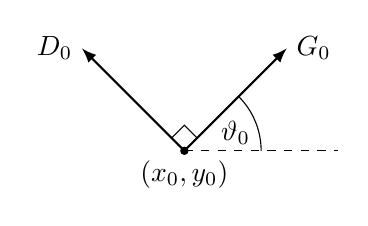
\begin{tikzpicture}[scale=0.65]
  % koordinate
  \coordinate (A) at (0, 0);
  \coordinate (B) at (2, 2);
  \coordinate (C) at (-2, 2);
  % vektorji
  \draw [-latex, black, thick, >=] (A) -- (B);
  \draw [-latex, black, thick, >=] (A) -- (C);
  % črte
  \draw [dashed] (0, 0) -- (3, 0);
  \draw [domain=0:45] plot ({1.5*cos(\x)}, {1.5*sin(\x)});
  \draw (0.25, 0.25) -- (0, 0.5) -- (-0.25, 0.25);
  % oznake
  \draw [fill=black] (A) circle (2pt) node [below] {$(x_0, y_0)$};
  \draw (B) node [right] {$G_0$};
  \draw (C) node [left] {$D_0$};
  \node (none) at (1, 0.35) {$\vartheta_0$};
  \end{tikzpicture}
}
%
\subfigure[V drugi točki $(x_1, y_1)$ imamo dve normalni smeri na gradient: $\vartheta_1 - \frac{\pi}{2}$ in $\vartheta_1 + \frac{\pi}{2}$. Izbrali smo $D_1$, da zmanjšamo ukrivljenost krivulje.]{
  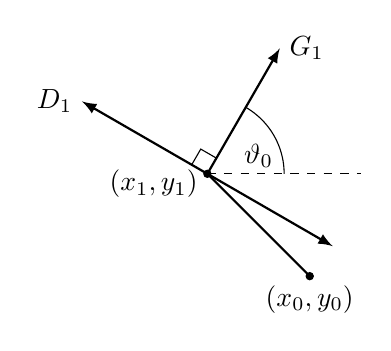
\begin{tikzpicture}[scale=0.65]
  % koordinate
  \coordinate (A) at (0, 0);
  \coordinate (B) at (-2, 2);
  \coordinate (C) at ({-2 + sqrt(8)*cos(60)}, {2 + sqrt(8)*sin(60)});
  \coordinate (D) at ({-2 + sqrt(8)*cos(150)}, {2 + sqrt(8)*sin(150)}); 
  \coordinate (E) at ({-2 + sqrt(8)*cos(-30)}, {2 + sqrt(8)*sin(-30)});
  % vektorji
  \draw [-latex, black, thick, >=] (B) -- (C);
  \draw [-latex, black, thick, >=] (B) -- (D);
  \draw [-latex, black, thick, >=] (B) -- (E);
  % črte
  \draw [dashed] (-2, 2) -- (1, 2);
  \draw [solid, thick] (A) -- (B);
  \draw [domain=0:60] plot ({-2 + 1.5*cos(\x)}, {2 + 1.5*sin(\x)});
  \draw ({-2 + sqrt(0.125)*cos(150)}, {2 + sqrt(0.125)*sin(150)})
        -- ({-2 + sqrt(0.25)*cos(105)}, {2 + sqrt(0.25)*sin(105)})
        -- ({-2 + sqrt(0.125)*cos(60)}, {2 + sqrt(0.125)*sin(60)});
  % oznake
  \draw [fill=black] (B) circle (2pt);
  \draw [fill=black] (A) circle (2pt) node [below] {$(x_0, y_0)$};
  \draw (-2, 1.8) node [left] {$(x_1, y_1)$};
  \draw (C) node [right] {$G_1$};
  \draw (D) node [left] {$D_1$};
  \node (none) at (-1, 2.35) {$\vartheta_0$};
  \end{tikzpicture}
}
%
\subfigure[Ta postopek ponavljamo pri iskanju ostalih kontrolnih točk. Potezo čopiča bomo upodobili kot kubični $B$-zlepek s kontrolnimi točkami $(x_i, y_i)$. Razdalja med kontrolnimi točkami je enaka trenutnemu polmeru čopiča.]{
  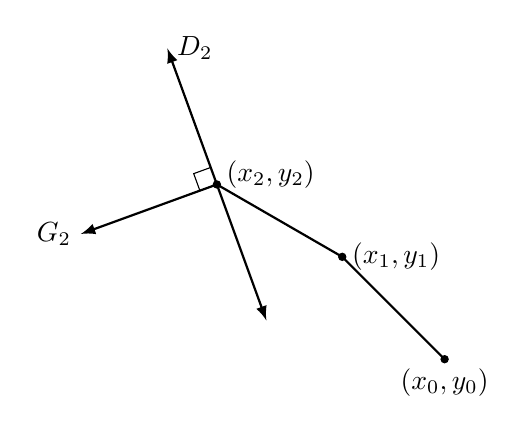
\begin{tikzpicture}[scale=0.65]
  % koordinate
  \coordinate (A) at (0, 0);
  \coordinate (B) at (-2, 2);
  \coordinate (C) at ({-2 + sqrt(8)*cos(150)}, {2 + sqrt(8)*sin(150)});
  \coordinate (D) at ({-2 + sqrt(8)*cos(150) + sqrt(8)*cos(110)}, {2 + sqrt(8)*sin(150) + sqrt(8)*sin(110)});
  \coordinate (E) at ({-2 + sqrt(8)*cos(150) + sqrt(8)*cos(200)}, {2 + sqrt(8)*sin(150) + sqrt(8)*sin(200)});
  \coordinate (F) at ({-2 + sqrt(8)*cos(150) + sqrt(8)*cos(290)}, {2 + sqrt(8)*sin(150) + sqrt(8)*sin(290)}); 
  % vektorji
  \draw [-latex, black, thick, >=] (C) -- (D);
  \draw [-latex, black, thick, >=] (C) -- (E);
  \draw [-latex, black, thick, >=] (C) -- (F);
  % črte
  \draw [solid, thick] (A) -- (B) -- (C);
  \draw ({-2 + sqrt(8)*cos(150) + sqrt(0.125)*cos(110)}, {2 + sqrt(8)*sin(150) + sqrt(0.125)*sin(110)})
        -- ({-2 + sqrt(8)*cos(150) + sqrt(0.25)*cos(155)}, {2 + sqrt(8)*sin(150) + sqrt(0.25)*sin(155)})
        -- ({-2 + sqrt(8)*cos(150) + sqrt(0.125)*cos(200)}, {2 + sqrt(8)*sin(150) + sqrt(0.125)*sin(200)});
  % oznake
  \draw [fill=black] (A) circle (2pt) node [below] {$(x_0, y_0)$};
  \draw [fill=black] (B) circle (2pt) node [right] {$(x_1, y_1)$};
  \draw [fill=black] (C) circle (2pt);
  \draw ({-2 + sqrt(8)*cos(150)}, {2.2 + sqrt(8)*sin(150)}) node [right] {$(x_2, y_2)$};
  \draw (D) node [right] {$D_2$};
  \draw (E) node [left] {$G_2$};
  \end{tikzpicture}
}
%
\caption{Iskanje novih kontrolnih točk.}
\label{fig:kontrolneTocke}
\end{figure}
%
Ukrivljenost krivulje lahko nadziramo s %TODO prevod
infinite impulse response filter na smer poteze. Filter kontroliramo z vnaprej določeno filtrirno konstanto $f_c$.  Za dano zadnjo smer $D_{i-1}' = (d_{x, i-1}', d_{y, i-1}')$ in trenutno smer poteze $D_i = (d_x, d_y)$ izračunamo filtrirano smer kot
$$D_i' = f_c D_i + (1 - f_c) D_{i-1}' = (f_c d_{x, i} + (1 - f_c) d_{x, i-1}', f_c d_{y, i} + (1 - f_c) d_{y, i-1}').$$ 
%
V algoritmu \ref{alg:splineStroke} je podana psevdokoda za iskanje kontrolnih točk.

%
\begin{algorithm}[htb]
  \caption{Iskanje kontrolnih točk za kubični $B$-zlepek..}
  \label{alg:splineStroke}
\begin{algorithmic}[1]
\Require $x_0$ $y_0$, $R$, $G$
\Ensure Seznam kontrolnih točk $K$.
\Function {Poteza} {$x_0$, $y_0$, $R$, $G$}
  \State $C$ $\gets$ $G.barva(x_0, y_0)$ % TODO \gets
  \State $K$ $\leftarrow$ prazen seznam kontrolnih točk
  \State Dodamo točko $(x_0, y_0)$ v seznam kontrolnih točk $K$.
  \State $(x, y)$ $\leftarrow$ $(x_0, y_0)$
  \State $(zd_x, zd_y)$ $\leftarrow$ $(0, 0)$
  \For {$i \in [1, \ldots, l_{max}]$}
    \If {$i > l_{min}$ $\And$ $\abs{G.barva(x, y) - P.barva(x, y)} < \abs{G.barva(x, y) - C}$} % TODO zakaj ne dela \And? 
      \State \Return $K$
    \EndIf
    \If {$G.magnituda(x, y) == 0$}
      \State \Return $K$
    \EndIf
    \State $(g_x, g_y)$ $\gets$ $G.smer(x, y)$
    \State $(d_x, d_y)$ $\gets$ $(-g_y, g_x)$
    \If {$zd_x \cdot d_x + zd_y \cdot d_y < 0$}
      \State $(d_x, d_y) = (-d_x, -d_y)$
    \EndIf
    \State
    \State $(d_x, d_y) = f_c \cdot (d_x, d_y) + (1 - f_c) \cdot (zd_x, zd_y)$
    \State $(d_x, d_y) = (d_x, d_y) / \sqrt{d_x^2 + d_y^2}$
    \State $(x, y) = (x + R \cdot d_x, y + R \cdot d_y)$
    \State $(zd_x, zd_y) = (d_x, d_y)$
    \State Točko $(x, y)$ dodamu seznamu $K$.
  \EndFor
\EndFunction
\end{algorithmic}
\end{algorithm}
%
Minimalno dolžino za potezo $l_{min}$ predpišemo, da se izognemo prekratkim potezam, ki bi delovale moteče. Za upodabljanje potez najprej s pomočjo subdivizij izračunamo zlepek. Nato pa vzdolž poti dobljenega zlepka narišemo potezo z antialiazirano ciklično masko.
%
\section{Anizotropični čopič za likovno upodabljanje}
Likovno upodabljanje s čopičem sestoji iz teh glavnih sklopov:
%
\begin{itemize}
  \item postavitev potez na platno in njihovi parametri (velikost, prosojnost \ldots);
  \item izračun vektorskega polja, ki določi smeri potez in njihovo pot (množica urejenih točk);
  \item upodabljanje potez čopiča, ki pove kako bomo posamezno potezo upodobili na platnu.
\end{itemize}
%
Pogledali si bomo upodabljanje potez s čopičem.
%
\subsection{Upodabljanje potez z anizotropičnim čopičem}
Najpogostejša metoda za upodabljanje potez je risanje antialiazirane črte vzdolž poti poteze. Čeprav je to enostavno za implementacijo, pa se na ta način upodobljene poteze od ročno narisanih potez s čopičem močno razlikujejo. Antialiazirana črta ima le eno barvo, brez strukture. Predstavili bomo simulacijo ročnega risanja s čopičem. Najprej bomo predstavili model anizotropičnega čopiča. V maski čopiča bo vsaka vrednost večja od 0 predstavljala pripadajočo nit na čopiču. Inteziteta posameznih elemntov maske predstavljajo kontakt med niti čopiča in platnom (0 pomeni, da stika ni; 1 pomeni, da je popolni kontakt). Prosojnost čopiča je določena kot povprečna vrednost intezitet v maski čopiča. Vsaki niti čopiča najprej predpišemo barvo in nato vlečemo masko čopiča vzdolž poti poteze.

Digitalni čopič, ki smo ga opislai zgoraj nastavimo v treh korakih:
%
\begin{enumerate}
  \item Izbrati moramo pravo velikost maske za čopič ali pa dano masko za čopiča skalirati, da ta ustreza velikosti čopiča.
  \item Intezitete v maski čopiča pomnožimo s parametrom, ki smo ga nastavili, da prilagodimo inteziteto čopiča.
  \item Posameznim nitim čopiča v maski čopiča priredimo barvo (barvo priredimo le tistim elemntom maske, ki imajo vrednost večjo od 0).
\end{enumerate}
% 
Barvo posameznim nitim čopiča določimo s formulo
$$
C_{nit} = \alpha \cdot C_{nit} + (1 - \alpha) \cdot C_{poteza} + C_{"sum},
$$
kjer je $C_{nit}$ barva na referenčni sliki, $C_{poteza}$ je barva začetne kontrolne točke za potezo in $C_{"sum}$ je perturbacija barve, s katero dosežemo učinek približnosti pri slikanju.

Po inicializaciji čopiča, narišemo potezo čopiča vzdolž poti, ki je sestavljena iz urejenih točk. Natančneje, na vsaki točki postavimo našo masko in pobarvamo območje, ki ga zavzema maska na sliki po formuli
$$
C_{platno} = \frac{I_{nit}}{255} \cdot C_{nit} + (1 - \frac{I_{nit}}{255} \cdot C_{platno}),
$$
kjer je $C_{platno}$ matrika barv ustreznega območja na platnu in je $I_{nit}$ maska čopiča z intezitetami 
%
\subsection{Lighting effect} % TODO
Dodajanje učinka svetlosti in bleščanja platnu, lahko zelo izpopolni kvaliteto upodabljanja slik. Predstavili bomo metodo za dodajanje efekta svetljenja, ki je za implementacijo zelo enostavna. Podobno kot Hertzmann v \ref[7], moramo najprej naračunati višinsko polje za platno, ki za vsako slikovno točko na platnu predstavlja njeno višino. Za razliko od Hertzmanna, ki vsaki posamezni potezi predpiše preslikavi, ki določata prosojnost in višino posameznih slikovnih točk na potezi, bomo uporabili masko čopiča in antialiazirano črto ter z upodabljanjem določili višinsko in prosojnostno preslikavo.

Inteziteto posameznih slikovnih točk na potezi čopiča (višinska preslikava), določimo kot povprečno vrednost intezitet, ki pri risanju s čopičem prečkajo to slikovno točko. Prosojnostno preslikavo pa določimo z upodobitvijo poteze čopiča na črno podlago kot antialiazirano črto, kateri nastavimo polmer nekoliko manj od polemra čopiča. Prosojnostne preslikave posameznih potez nato uporabimo kot uteži pri izračunu višinskega polja za platno.

Namesto uporabe Modela za senčenje Phong, bomo simulirali lighting effect % TODO prevod
tako, da bomo prilagodili intezitete slikovnih točk na platnu. Za vsako slikovno točko $(x, y)$ na platnu, je prilagoditev intezitete te točke sorazmerna z višinsko razliko $D(x, y)$
%
\begin{align*}
d & = O(x, y) - \pi/2, \\
D(x, y) & = h(x + \cos d, y + \sin d) - h(x, y),
\end{align*}
%
kjer $d$ predstavlja smer, ki je pravokotna na orientacijo poteze $O(x, y)$ in  $h$ označuje višino slikovne točke, tj.\ pripadajočo inteziteto slikovne točke na višinskem polju platna. Če je $D(x, y)$ pozitiven, potem bo vrednost intezitete slikovne točke narasla, sicer bo padla. Prilagoditev intezitet mora biti majhna vrednost, v primeru, ko je vrednost intezitete blizu 0 ali 255, po drugi strani je vrednost prilagoditve lahko ogromna, kadar je začetna vrednost intezitete blizu povprečne vrednosti 127. Natančneje, za slikovno točko $(x, y)$ na platnu, prilagoditev intezitet izračunamo kot
$$
I(x, y) = I(x, y) + a \cdot D(x, y) \cdot \frac{\min (I(x, y), 255 - I(x, y))}{127.5},
$$
kjer je $a$ parameter, s katerim kontroliramo inteziteto lightinga. %TODO prevod
Ker je platno barvno, prilagoditev intezitete izvedemo za vsak barvni kanala posebaj.
%
\subsection{Fast paint texture}
Algoritem za vhod dobi urejen seznam potez čopiča, model senčenja in množico višinskih polj potez čopiča. Likovno upodabljanje tako poteka v treh korakih:
%
\begin{enumerate}
  \item S kompoziranjem potez čopiča najprej izračunamo osnovno sliko.
  \item Izračunamo višinsko polje, tj.\ za vsako slikovno točko na sliki pove skupno višino nanešene barve.
  \item Končno sliko izračunamo s pomočjo bump-mappinga s pomočjo modela senčenja Phong.
\end{enumerate}
%
Najprej moramo ustvariti matriko z vrednostmi barv, ki jih ima slika brez svetljenja. To naredimo s kompoziranjem potez čopiča na platno.

Sedaj izračunamo višinsko polje, ki pove višino nanešene barve za posamezne točke. Najprej nastavimo polje z ustreznimi dimenzijami in nastavimo barvo na črno. nato v vrstnem redu upodabljamo poteze čopiča, ampak kot črnobele. Toni slikovnih točk poteze so določeni s teksturno preslikavo. Vsakič celotni potezi dodamo zraven še vrednost, ki je sorazmerna s številom potez čopiča, ki so že narisane. Zato so poteze, ki so v ozadju narisane bolj temno (tj.\ plitva območja oz.\ dolince), poteze naisane kasneje pa bodo bolj svetlih barv. Če bi višinsko polje gradili tako, da bi kar prištevali zraven višine novo narisanih potez, bi se poteze narisane v ozadju pojavljale v višinskem polju, česar pane želimo.

Končno sliko izračunamo iz višinskega polja in osnovne slikae tako, da za izračunamo polje normal iz višinskega polje in poračunamo nove barve s pomočjo modela Phong.
%
% Notes on Gaussian blur
% http://stackoverflow.com/questions/17841098/gaussian-blur-standard-deviation-radius-and-kernel-size

% Z-buffer
% http://www.google.si/url?sa=t&rct=j&q=&esrc=s&source=web&cd=15&ved=0C
% JgBEBYwDg&url=http%3A%2F%2Fweb.eecs.utk.edu%2F~huangj%2Fcs456%2
% Fnotes%2F456_rasterization.pdf&ei=6WRuUuIYita0BoaZgZgH&usg=AFQjCNHgr
% Ig6qcQ3zXtszjawy9pEos0owQ&sig2=S1eiksIjOd80pAukxEv7xg&bvm=bv.5512
% 3115,d.Yms